\documentclass[landscape,a0paper,final,showframe]{baposter}

\usepackage{times}
\usepackage{calc}
\usepackage{graphicx}
\usepackage{amsmath}
\usepackage{amssymb}
\usepackage{relsize}
\usepackage{multirow}
\usepackage{bm}

%%---------Añadidas por Jenni
\usepackage[spanish]{babel} 
\usepackage[utf8]{inputenc}
\usepackage{listings}
\usepackage{color}
\usepackage[T1]{fontenc}
\usepackage{graphicx}
\usepackage{multicol}
\usepackage{url}
%%..........fin de mis adiciones
\usepackage{pgfbaselayers}
\pgfdeclarelayer{background}
\pgfdeclarelayer{foreground}
\pgfsetlayers{background,main,foreground}

\usepackage{helvet}
%\usepackage{bookman}
\usepackage{palatino}

\newcommand{\captionfont}{\footnotesize}

\selectcolormodel{cmyk}

\graphicspath{{images/}}

%%%%%%%%%%%%%%%%%%%%%%%%%%%%%%%%%%%%%%%%%%%%%%%%%%%%%%%%%%%%%%%%%%%%%%%%%%%%%%%%
%%%% Some math symbols used in the text
%%%%%%%%%%%%%%%%%%%%%%%%%%%%%%%%%%%%%%%%%%%%%%%%%%%%%%%%%%%%%%%%%%%%%%%%%%%%%%%%
% Format 
\newcommand{\Matrix}[1]{\begin{bmatrix} #1 \end{bmatrix}}
\newcommand{\Vector}[1]{\Matrix{#1}}
\newcommand*{\SET}[1]  {\ensuremath{\mathcal{#1}}}
\newcommand*{\MAT}[1]  {\ensuremath{\mathbf{#1}}}
\newcommand*{\VEC}[1]  {\ensuremath{\bm{#1}}}
\newcommand*{\CONST}[1]{\ensuremath{\mathit{#1}}}
\newcommand*{\norm}[1]{\mathopen\| #1 \mathclose\|}% use instead of $\|x\|$
\newcommand*{\abs}[1]{\mathopen| #1 \mathclose|}% use instead of $\|x\|$
\newcommand*{\absLR}[1]{\left| #1 \right|}% use instead of $\|x\|$

\def\norm#1{\mathopen\| #1 \mathclose\|}% use instead of $\|x\|$
\newcommand{\normLR}[1]{\left\| #1 \right\|}% use instead of $\|x\|$

%%%%%%%%%%%%%%%%%%%%%%%%%%%%%%%%%%%%%%%%%%%%%%%%%%%%%%%%%%%%%%%%%%%%%%%%%%%%%%%%
% Multicol Settings
%%%%%%%%%%%%%%%%%%%%%%%%%%%%%%%%%%%%%%%%%%%%%%%%%%%%%%%%%%%%%%%%%%%%%%%%%%%%%%%%
\setlength{\columnsep}{0.7em}
\setlength{\columnseprule}{0mm}


%%%%%%%%%%%%%%%%%%%%%%%%%%%%%%%%%%%%%%%%%%%%%%%%%%%%%%%%%%%%%%%%%%%%%%%%%%%%%%%%
% Save space in lists. Use this after the opening of the list
%%%%%%%%%%%%%%%%%%%%%%%%%%%%%%%%%%%%%%%%%%%%%%%%%%%%%%%%%%%%%%%%%%%%%%%%%%%%%%%%
\newcommand{\compresslist}{%
\setlength{\itemsep}{1pt}%
\setlength{\parskip}{0pt}%
\setlength{\parsep}{0pt}%
}


%%%%%%%%%%%%%%%%%%%%%%%%%%%%%%%%%%%%%%%%%%%%%%%%%%%%%%%%%%%%%%%%%%%%%%%%%%%%%%
%%% Begin of Document
%%%%%%%%%%%%%%%%%%%%%%%%%%%%%%%%%%%%%%%%%%%%%%%%%%%%%%%%%%%%%%%%%%%%%%%%%%%%%%

\begin{document}

%%%%%%%%%%%%%%%%%%%%%%%%%%%%%%%%%%%%%%%%%%%%%%%%%%%%%%%%%%%%%%%%%%%%%%%%%%%%%%
%%% Here starts the poster
%%%---------------------------------------------------------------------------
%%% Format it to your taste with the options
%%%%%%%%%%%%%%%%%%%%%%%%%%%%%%%%%%%%%%%%%%%%%%%%%%%%%%%%%%%%%%%%%%%%%%%%%%%%%%
\typeout{Poster Starts}
\background{
  \begin{tikzpicture}[remember picture,overlay]%
    \draw (current page.north west)+(-2em,-0em) node[anchor=north west] {\hspace{-2em}\includegraphics[height=1.1\textheight]{silhouettes_background}};
  \end{tikzpicture}%
}
\definecolor{silver}{cmyk}{0,0,0,0.3}
\definecolor{yellow}{cmyk}{0,0,0.9,0.0}
\definecolor{reddishyellow}{cmyk}{0,0.22,1.0,0.0}
\definecolor{black}{cmyk}{0,0,0.0,1.0}
\definecolor{darkYellow}{cmyk}{0,0,1.0,0.5}
\definecolor{darkSilver}{cmyk}{0,0,0,0.1}

\definecolor{lightyellow}{cmyk}{0,0,0.3,0.0}
\definecolor{lighteryellow}{cmyk}{0,0,0.1,0.0}
\definecolor{lighteryellow}{cmyk}{0,0,0.1,0.0}
\definecolor{lightestyellow}{cmyk}{0,0,0.05,0.0}
\begin{poster}{
  % Show grid to help with alignment
  grid=false,
  % Column spacing
  colspacing=1em,
  % Color style
  bgColorOne=lighteryellow,
  bgColorTwo=lightestyellow,
  borderColor=reddishyellow,
  headerColorOne=yellow,
  headerColorTwo=reddishyellow,
  headerFontColor=black,
  boxColorOne=lightyellow,
  boxColorTwo=lighteryellow,
  % Format of textbox
  textborder=roundedleft,
  % Format of text header
  eyecatcher=false,
  headerborder=open,
  headerheight=0.08\textheight,
  headershape=roundedright,
  headershade=plain,
  headerfont=\Large\textsf, %Sans Serif
  boxshade=plain,
%  background=shade-tb,
  background=plain,
  linewidth=2pt
  }
  % Eye Catcher
  {} % No eye catcher for this poster. If an eye catcher is present, the title is centered between eye-catcher and logo.
  % Title
  {\sf %Sans Serif
  %\bf% Serif
  Python con Baterías Incluídas}
  % Authors
  {\sf %Sans Serif
  % Serif
  Jennifer Maldonado\hspace{3em}
  Caracas, Venezuela
  }
  % Python logo
  {{\begin{minipage}{16em}
    \hfill
    
\includegraphics[height=7em]{python_logo}
  \end{minipage}}
  }

  \tikzstyle{light shaded}=[top color=baposterBGtwo!30!white,bottom color=baposterBGone!30!white,shading=axis,shading angle=30]

  % Width of left inset image
     \newlength{\leftimgwidth}
     \setlength{\leftimgwidth}{0.78em+8.0em}

%%%%%%%%%%%%%%%%%%%%%%%%%%%%%%%%%%%%%%%%%%%%%%%%%%%%%%%%%%%%%%%%%%%%%%%%%%%%%%
%%% Now define the boxes that make up the poster
%%%---------------------------------------------------------------------------
%%% Each box has a name and can be placed absolutely or relatively.
%%% The only inconvenience is that you can only specify a relative position 
%%% towards an already declared box. So if you have a box attached to the 
%%% bottom, one to the top and a third one which should be in between, you 
%%% have to specify the top and bottom boxes before you specify the middle 
%%% box.
%%%%%%%%%%%%%%%%%%%%%%%%%%%%%%%%%%%%%%%%%%%%%%%%%%%%%%%%%%%%%%%%%%%%%%%%%%%%%%
    %
    % A coloured circle useful as a bullet with an adjustably strong filling
    \newcommand{\colouredcircle}[1]{%
      \tikz{\useasboundingbox (-0.2em,-0.32em) rectangle(0.2em,0.32em); \draw[draw=black,fill=baposterBGone!80!black!#1!white,line width=0.03em] (0,0) circle(0.18em);}}

%%%%%%%%%%%%%%%%%%%%%%%%%%%%%%%%%%%%%%%%%%%%%%%%%%%%%%%%%%%%%%%%%%%%%%%%%%%%%%
  \headerbox{Código pythonico}{name=filosofia,column=0,row=0}{
%%%%%%%%%%%%%%%%%%%%%%%%%%%%%%%%%%%%%%%%%%%%%%%%%%%%%%%%%%%%%%%%%%%%%%%%%%%%%%
   {}Entre los principios de python se encuentran la legibilidad y transparencia,
   por lo cual Tim Peters redactó el Zen de Python:
	{}
	\begin{itemize}
	\item Bello es Mejor que feo,  Explícito es Mejor que ímplicito. Simple es Mejor que complejo, Plano es Mejor que anidado.
	\item Disperso es mejor que denso, La legibilidad Cuenta. Los casos Especiales no son tan especiales para quebrantar las reglas.
	\item Aunque lo práctico gane a la pureza. Los errores nunca deberían dejarse pasar silenciosamente, A menos que hayan sido silenciados explícitamente.
	\item Frente a la ambigüedad, rechaza la tentación de adivinar. Debería haber una y preferiblemente solo una obvia manera de hacerlo. Aunque esa manera puede no ser obvia al principio a menos que usted sea holandés
	\item Ahora es mejor que nunca. Aunque nunca es a menudo mejor que ya mismo. Si la implementación es difícil de explicar, es una mala idea. Si la implementación es fácil de explicar, puede que sea una buena idea.
	\item Los espacios de nombres (namespaces) son una gran idea ¡Hagamos más de esas cosas!
	\end{itemize}
 }

%%%%%%%%%%%%%%%%%%%%%%%%%%%%%%%%%%%%%%%%%%%%%%%%%%%%%%%%%%%%%%%%%%%%%%%%%%%%%%
  \headerbox{Buenas Prácticas}{name=bestpractice,column=0,above=bottom,below=filosofia}{
%%%%%%%%%%%%%%%%%%%%%%%%%%%%%%%%%%%%%%%%%%%%%%%%%%%%%%%%%%%%%%%%%%%%%%%%%%%%%%
	\begin{itemize}
		\item Tomar en cuenta el Zen de python.
		\item virtualenv: Permite crear entornos virtuales para python, de forma que tengas aislado el core de python y realizar pruebas de despliegues, para instalar los paquetes necesarios, sin alterar el python del sistema, este paquete se puede encontrar en la biblioteca pypi.
		\item pep8: Es la guía de estilo para el código de python, Esto indica las convenciones, estandares, fue creado por Guido y modificada por Barry. Entre una de las convenciones es usar 4 espacios por nivel de identación, en las funciones alinear con el delimitador con el que fue abierto. Para más info: \\  \url{http://www.python.org/dev/peps/pep-0008/}
	\end{itemize}
  }

%%%%%%%%%%%%%%%%%%%%%%%%%%%%%%%%%%%%%%%%%%%%%%%%%%%%%%%%%%%%%%%%%%%%%%%%%%%%%%
  \headerbox{Extendiendo con Python}{name=extpython neutralization,column=1,row=0}{
%%%%%%%%%%%%%%%%%%%%%%%%%%%%%%%%%%%%%%%%%%%%%%%%%%%%%%%%%%%%%%%%%%%%%%%%%%%%%%
  \begin{multicols}{2}
	{\smaller Blender es una aplicación de diseño 3D, que permite extender su funcionalidad a través de scripts de python que complementan y facilitan rápido  uso, En este proyecto participan chicas como desarrolladoras: Andrea Weikert, Sandra Gilbert, entre otras. Además en Gimp también se puede extender mediante la cónsola de python, y permite añadir nuevos plugins para facilitar su uso, entre las chicas activas en el desarrollo y entrenamiento tenemos a: Alexia Death, Akkana Peck, entre otras. }
  \end{multicols}

  \begin{tabular}[t]{lr}
	    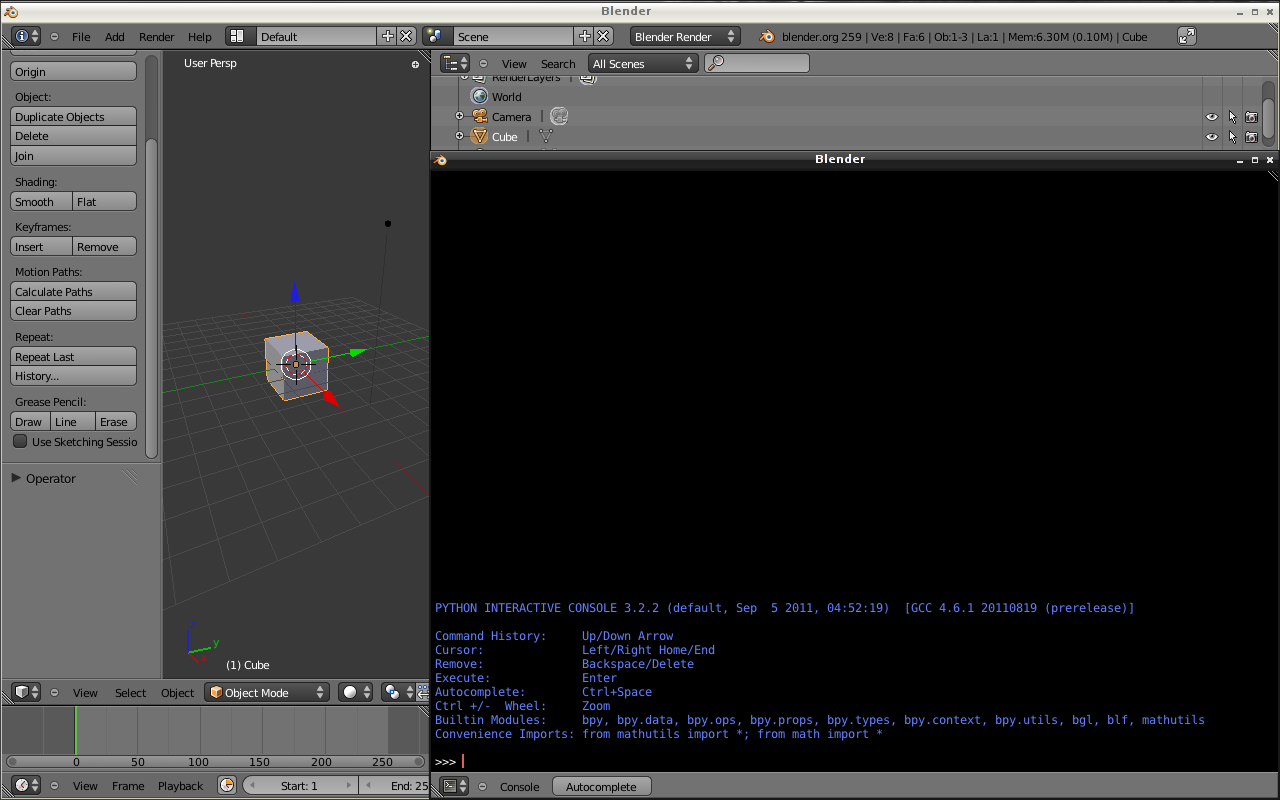
\includegraphics[width=3.5cm,height=2.5cm]{blender} &
	    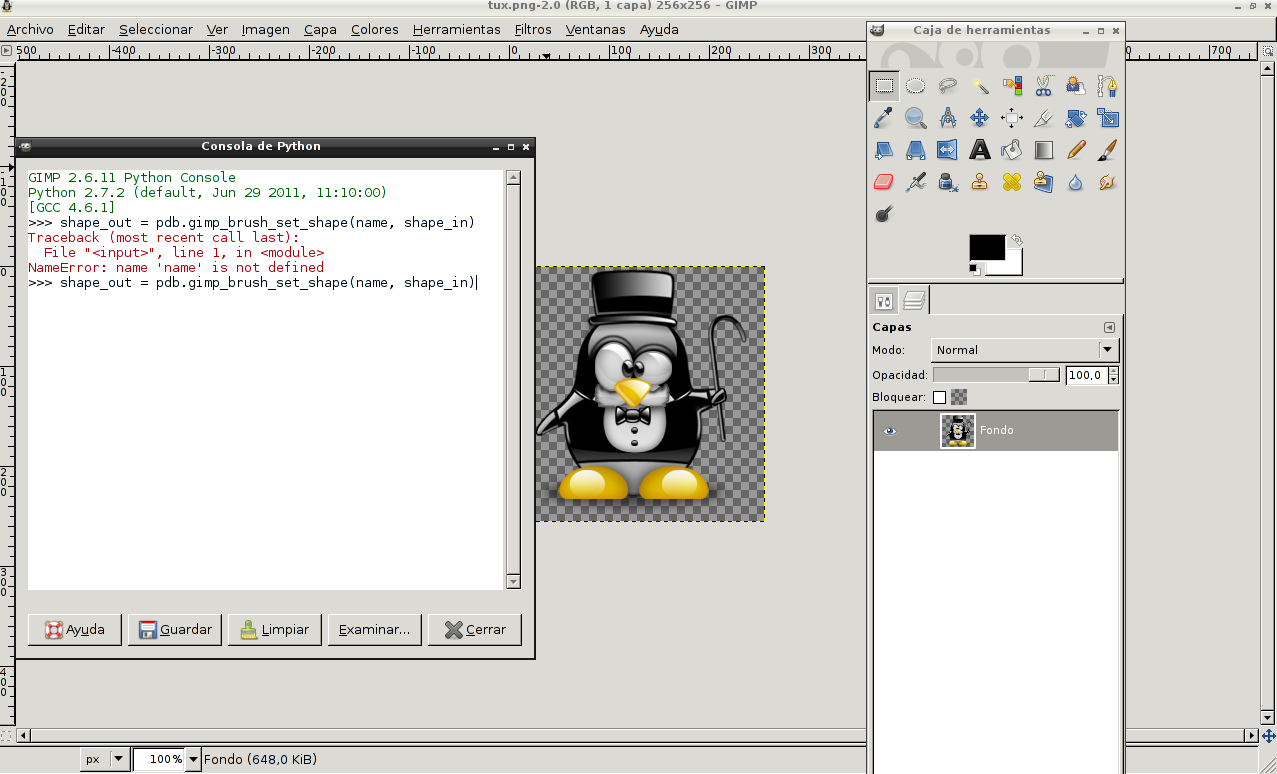
\includegraphics[width=3.5cm,height=2.5cm]{gimp}  
  \end{tabular}
  }
%%%%%%%%%%%%%%%%%%%%%%%%%%%%%%%%%%%%%%%%%%%%%%%%%%%%%%%%%%%%%%%%%%%%%%%%%%%%%%
  \headerbox{Aplicaciones Desarrolladas}{name=aplicacionpython,column=1,below=extpython neutralization,span=1,above=bottom}{
%%%%%%%%%%%%%%%%%%%%%%%%%%%%%%%%%%%%%%%%%%%%%%%%%%%%%%%%%%%%%%%%%%%%%%%%%%%%%%
  \begin{multicols}{2}
{\smaller Entre las aplicaciones desarrolladas con python se encuentran: calibre (un gestor de libros electrónicos)
		  Mercurial, Bazar (son control de version distribuidos), mailman (gestor de listas de correo),
 		  aplicaciones de escritorio como emesene (cliente de mensajería instantánea).
		  También python cuenta con un poderoso ORM llamado SQLalchemy, y frameworks
		  para el desarrollo web ágil, como Django, particularmente acá destacadan en la difusión sobre python y su desarrollo:
		  Audrey Roy, Christine Cheung, Esther Nam, Jessica Stanton, Katharine Jarmul, Sandy Strong,
		  Sophia Viklund, entre otras. Las chicas anteriormente nombradas forman parte de un grupo de usuarias llamado pyladies. 
	}
  \end{multicols}

  \begin{tabular}[t]{lp{1cm}lp{1cm}}
    
\includegraphics[height=2cm,width=2cm]{twisted} & 
    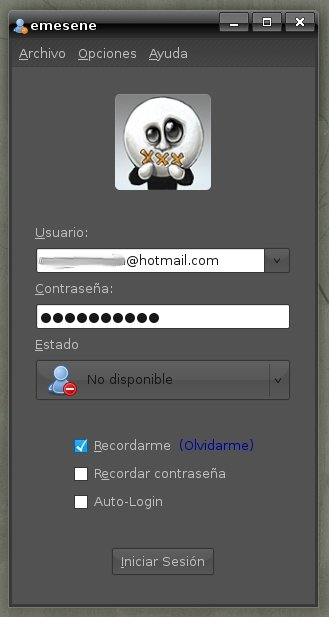
\includegraphics[height=2cm,width=2cm]{emesene} \\ 
    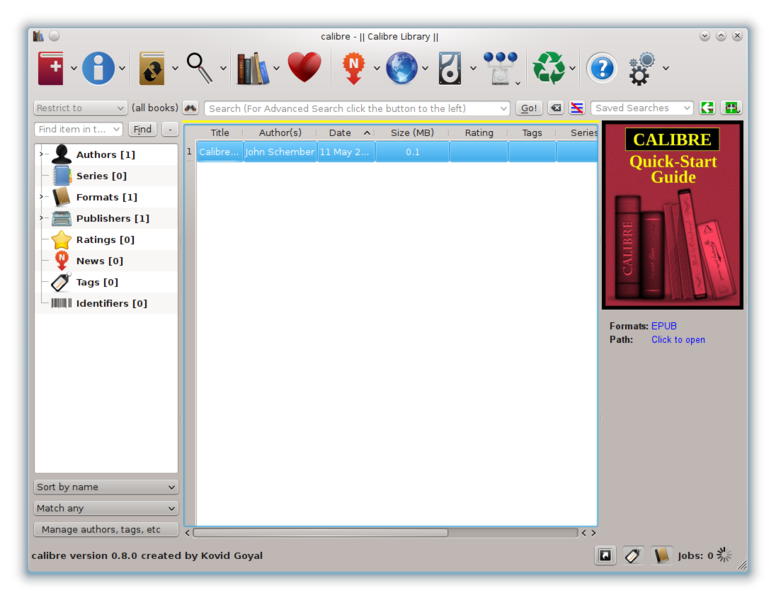
\includegraphics[height=3cm,width=2cm]{calibre} & 
    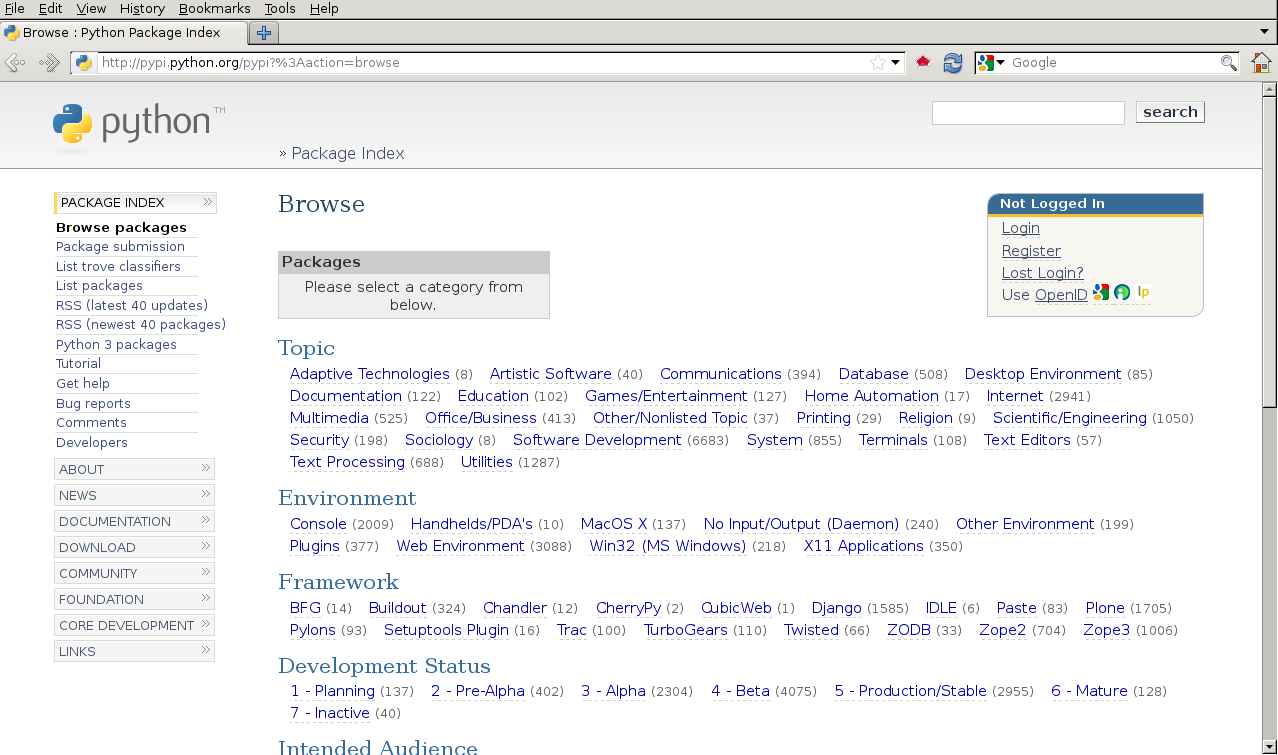
\includegraphics[height=2cm,width=2cm]{pypi} \\ 
    
\includegraphics[height=1cm,width=4cm]{django} & 
    
\includegraphics[height=1cm,width=3cm]{sqla-logo6} \\
  \end{tabular}
  }
%%%%%%%%%%%%%%%%%%%%%%%%%%%%%%%%%%%%%%%%%%%%%%%%%%%%%%%%%%%%%%%%%%%%%%%%%%%%%%
  \headerbox{¿De qué lenguajes de programación las personas están hablando?}{name=estadisticas,column=2,span=2,row=0}{
%%%%%%%%%%%%%%%%%%%%%%%%%%%%%%%%%%%%%%%%%%%%%%%%%%%%%%%%%%%%%%%%%%%%%%%%%%%%%%
      \begin{multicols}{2}
      Las gráficas mostradas a continuación fueron tomadas del sitio \url{http://langpop.com/}
      el cual muestra una variedad de data acerca de la popularidad de los 
      lenguajes de programación: 
      \end{multicols}\vspace{-1em}
      
      \begin{tabular}{ccc}
		\\
		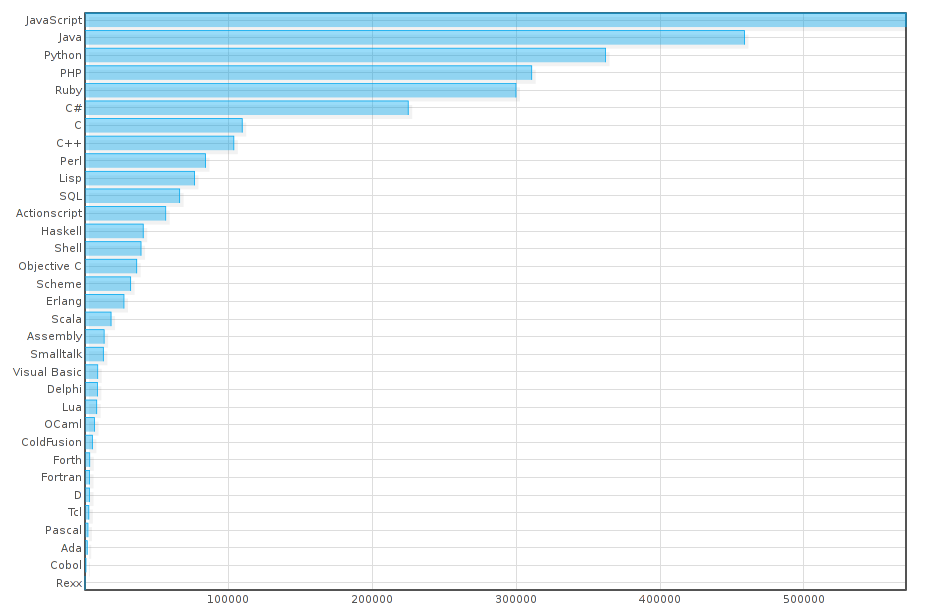
\includegraphics[height=0.20\linewidth]{delicious} &
		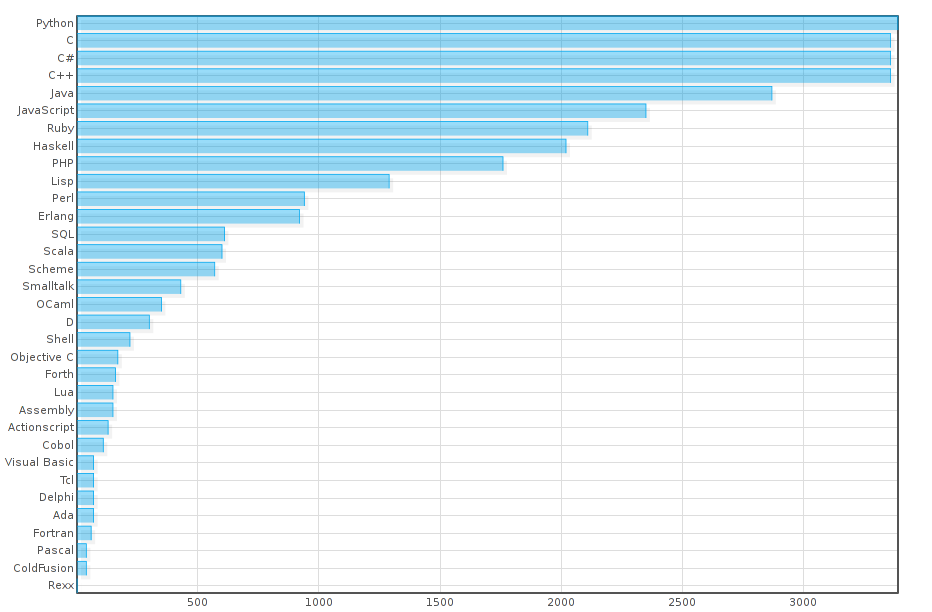
\includegraphics[height=0.20\linewidth]{programmingredit} &
		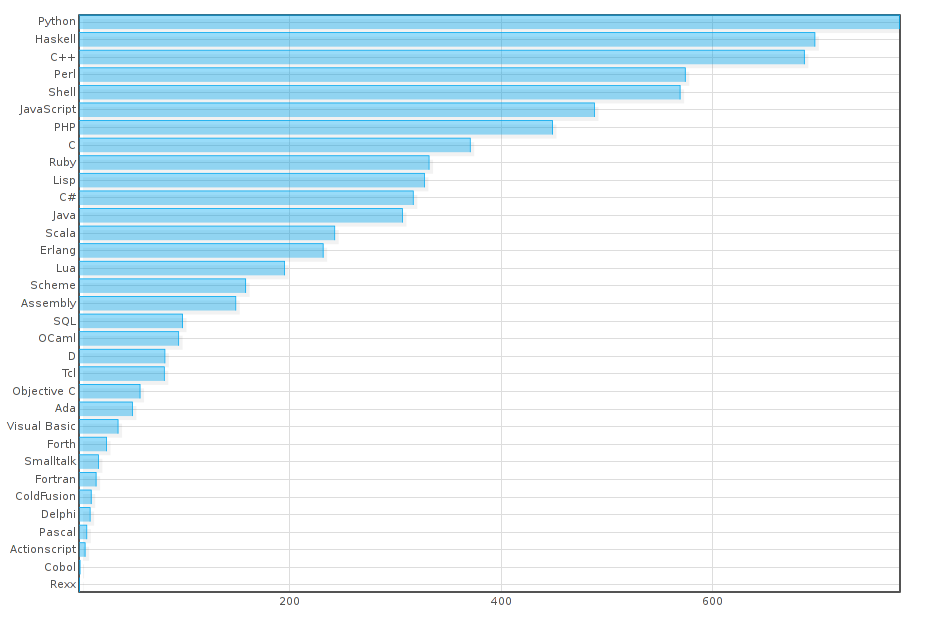
\includegraphics[height=0.20\linewidth]{irc} \\
		a) delicious &
		b) programming.reddit.com &
		c) IRC (bot)
      \end{tabular}\\
\\
  }%
%%%%%%%%%%%%%%%%%%%%%%%%%%%%%%%%%%%%%%%%%%%%%%%%%%%%%%%%%%%%%%%%%%%%%%%%%%%%%%
  \headerbox{En la variedad está el gusto}{name=sabores,column=2,span=1,above=bottom}{
%%%%%%%%%%%%%%%%%%%%%%%%%%%%%%%%%%%%%%%%%%%%%%%%%%%%%%%%%%%%%%%%%%%%%%%%%%%%%%
  {\setlength{\baselineskip}{0.4em}
  \smaller
  visita: \\
  \url{http://pyladies.com}\\
  \url{http://www.coactivate.org/projects/pyve/summary} o \url{http://www.coactivate.org/projects/ploneve/lists/ploneve-discussion} \\
  \url{http://mail.python.org/mailman/listinfo/python-es} \\
  \url{http://mail.python.org/mailman/listinfo/tutor} \\
  \url{http://www.python.org/community/lists/} \\ }
  }%

%%%%%%%%%%%%%%%%%%%%%%%%%%%%%%%%%%%%%%%%%%%%%%%%%%%%%%%%%%%%%%%%%%%%%%%%%%
   \headerbox{Tira cómica}{name=dibujo, column=2, span=1, row=1, below=estadisticas }{
%%%%%%%%%%%%%%%%%%%%%%%%%%%%%%%%%%%%%%%%%%%%%%%%%%%%%%%%%%%%%%%%%%%%%%%%%%
      \begin{tabular}{cc}
	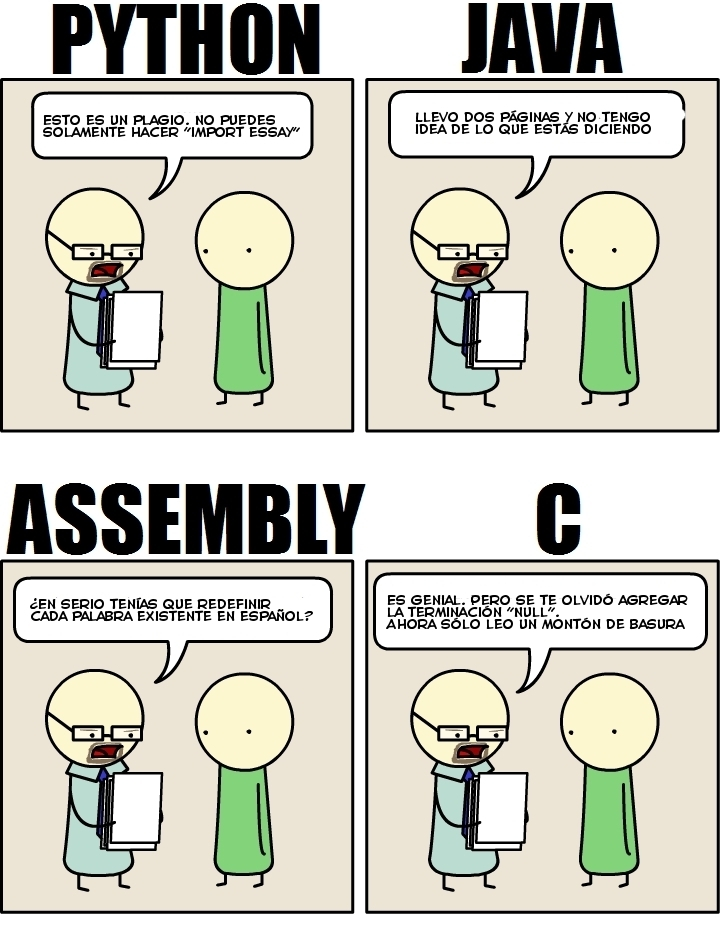
\includegraphics[height=4cm, width=3cm]{pythonrules1} &
	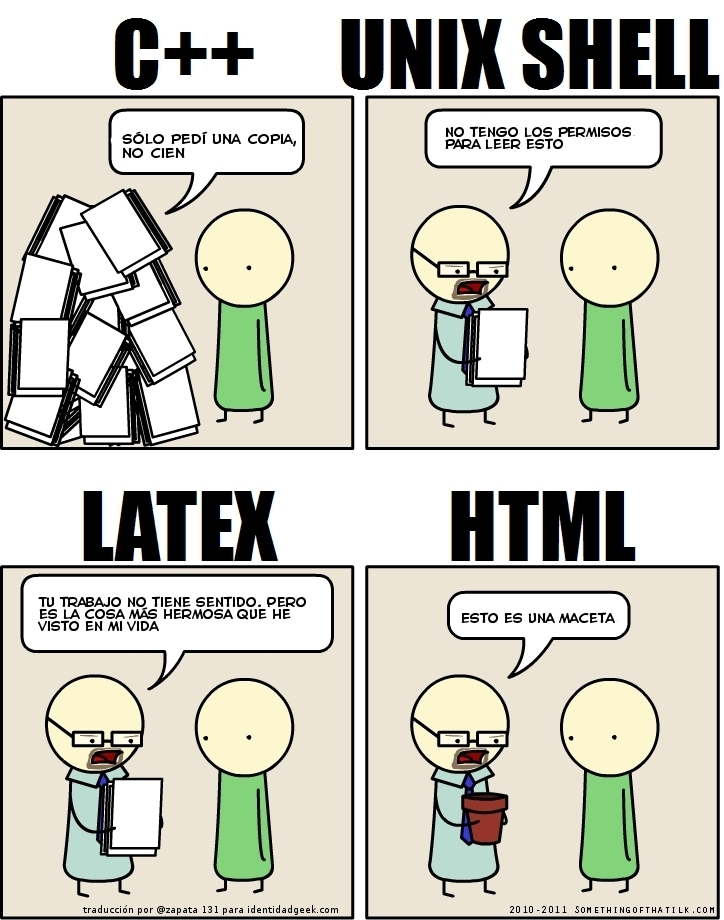
\includegraphics[height=4cm, width=3cm]{pythonrules2} \\
      \end{tabular}\\
   }


%%%%%%%%%%%%%%%%%%%%%%%%%%%%%%%%%%%%%%%%%%%%%%%%%%%%%%%%%%%%%%%%%%%%%%%%%%%%%%
  \headerbox{Pypi}{name=pypi,column=2, span=1,above=sabores, below=dibujo}{
%%%%%%%%%%%%%%%%%%%%%%%%%%%%%%%%%%%%%%%%%%%%%%%%%%%%%%%%%%%%%%%%%%%%%%%%%%%%%%
   Es una biblioteca de paquetes donde encontraremos un conjunto de aplicaciones
   para poder reutilizar conforme se requiera. Están clasificadas por diferentes tópicos
   como: Ambiente, Audiencia, Licencia, Frameworks, por sistema Operativo, entre otros. \\
   info: http://pypi.python.org \\
  }

%%%%%%%%%%%%%%%%%%%%%%%%%%%%%%%%%%%%%%%%%%%%%%%%%%%%%%%%%%%%%%%%%%%%%%%%%%%%%%
  \headerbox{Referencias}{name=references,column=3,above=bottom}{
%%%%%%%%%%%%%%%%%%%%%%%%%%%%%%%%%%%%%%%%%%%%%%%%%%%%%%%%%%%%%%%%%%%%%%%%%%%%%%
    \smaller
    \vspace{-0.4em}
    \bibliographystyle{ieee}
    \renewcommand{\section}[2]{\vskip 0.05em}
      \begin{thebibliography}{1}\itemsep=-0.01em
      \setlength{\baselineskip}{0.4em}
      \bibitem{amberg07:nonrigid}
	Página Oficial de Python
           \newblock http://www.python.org/ 
      \bibitem{amberg08:recognition}
        Group of women developers worldwide who love the Python programming language
           \newblock http://pyladies.com/
      \bibitem{amberg08:recognition}
	Python Venezuela
	   \newblock http://blog.pyve.org.ve/
      \bibitem{mvc}
	   Framework Django
           \newblock http://bit.ly/ooVCa6
      \bibitem{best}
	   PEP8
	   \newblock \url{http://www.python.org/dev/peps/pep-0008/}
      \bibitem{estadistica}
	   Popularidad de lenguajes
	   \newblock \url{http://langpop.com/}
      \bibitem{misceslaneos}
	   \newblock \url {http://geekfeminism.wikia.com/wiki/List\_of\_women\_in\_FLOSS}
      \bibitem{}
	   Curso de python por correo
	   \newblock \url {http://groups.google.com/group/curso-de-python-por-correo}
      \bibitem{}
	   Poster realizado con Latex Poster Template:
	   \newblock \url {http://www.brian-amberg.de/uni/poster/}
      \end{thebibliography}
  }%

%%%%%%%%%%%%%%%%%%%%%%%%%%%%%%%%%%%%%%%%%%%%%%%%%%%%%%%%%%%%%%%%%%%%%%%%%%%%%%
  \headerbox{Frameworks MVC}{name=mvc,column=3,below=estadisticas,above=references}{
%%%%%%%%%%%%%%%%%%%%%%%%%%%%%%%%%%%%%%%%%%%%%%%%%%%%%%%%%%%%%%%%%%%%%%%%%%%%%%
  Entre los más utilizados se encuentran: Django, Web2py, Pyramid, Web.py, Cubic Web y Zope 2.
  Otros no tan comunes: Grok, Pylons, TurboGears, Enamel, GAE framework, Gizmo, Glashammer, Nagare,
  notmm, Porcupine, Spyce, WHIFF, XPRESS.  
  \\
  \\
   Sin embargo el que posee más auge es Django, algunas de sus desarrolladoras son:
  Leah Culver, Audrey Roy, entre otras.
  Para más información visita:\\  https://www.djangoproject.com/ 
  \begin{tabular}{ccc}
	\\
	
\includegraphics[height=2cm, width=0.20\linewidth]{zope_only} &
	
\includegraphics[height=2cm, width=0.40\linewidth]{cubicweb} & 
	
\includegraphics[height=2cm, width=0.27\linewidth]{web2py}
  \end{tabular}
  }


%%%%%%%%%%%%%%%%%%%%%%%%%%%%%%%%%%%%%%%%%%%%%%%%%%%%%%%%%%%%%%%%%%%%%%%%%%%%%%
%%  \headerbox{Funding}{name=funding,column=3,span=1,above=bottom}{
%%%%%%%%%%%%%%%%%%%%%%%%%%%%%%%%%%%%%%%%%%%%%%%%%%%%%%%%%%%%%%%%%%%%%%%%%%%%%%
%%  \smaller 
%%  This work was supported in part by Microsoft Research through the European PhD Scholarship Programme.
%%  }%
\end{poster}%
%
\end{document}
